\subsection{Extreme Gradient Boosting}

\begin{frame}{Extreme Gradient Boosting}
    Intro
\end{frame}

\begin{frame}{Features}
    \begin{figure}[h]
		\centering
		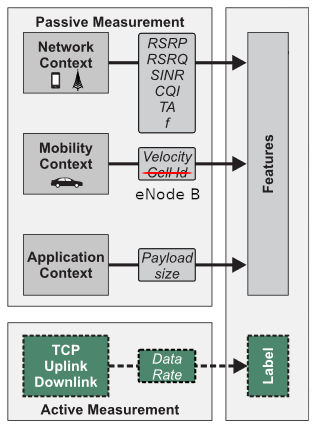
\includegraphics[height=0.75\textheight]{grafiken/features}
		\caption{Modellfeatures \cite{IEEE}.}
		\label{features}
	\end{figure}
\end{frame}

\begin{frame}{Tuning}
    Tuning
\end{frame}

\begin{frame}{Validierung}
	\begin{figure}[h]
		\centering
		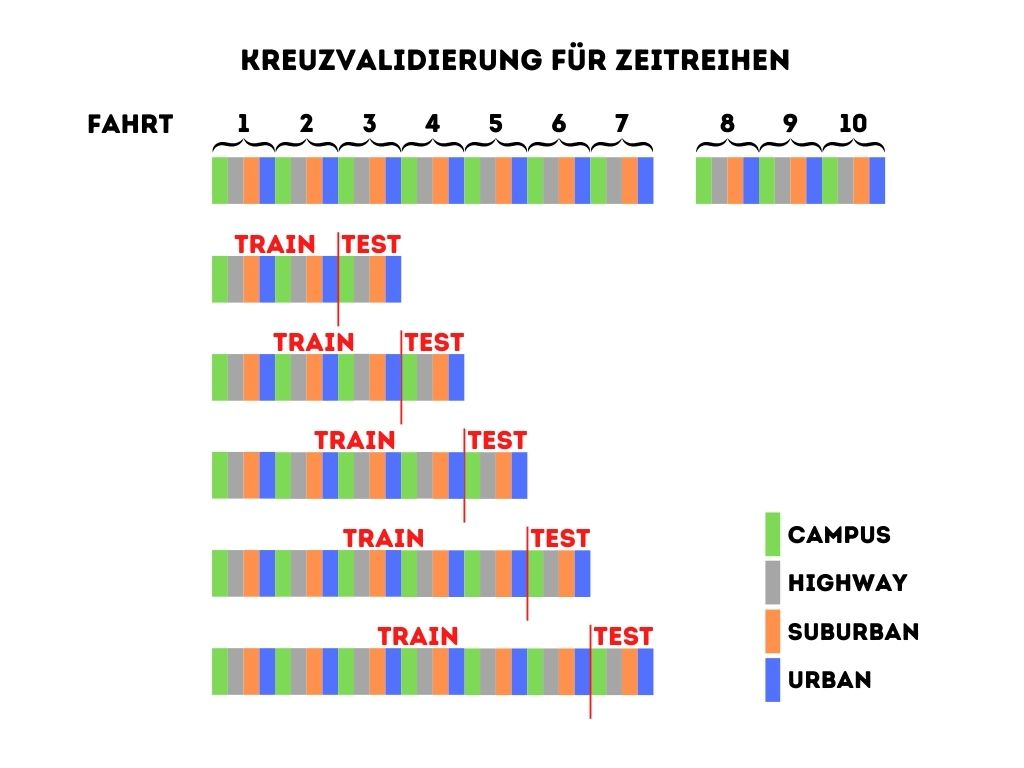
\includegraphics[scale=0.33]{kreuzvalidierung}
		\caption{Einteilungen in Trainings- und Testdatensätze bei der Kreuzvalidierung für Zeitreihen.}
		\label{kreuzvalidierung}
	\end{figure}
\end{frame}

\begin{frame}{Out-of-Sample Vorhersagen}
    \begin{figure}[h]
        \centering
        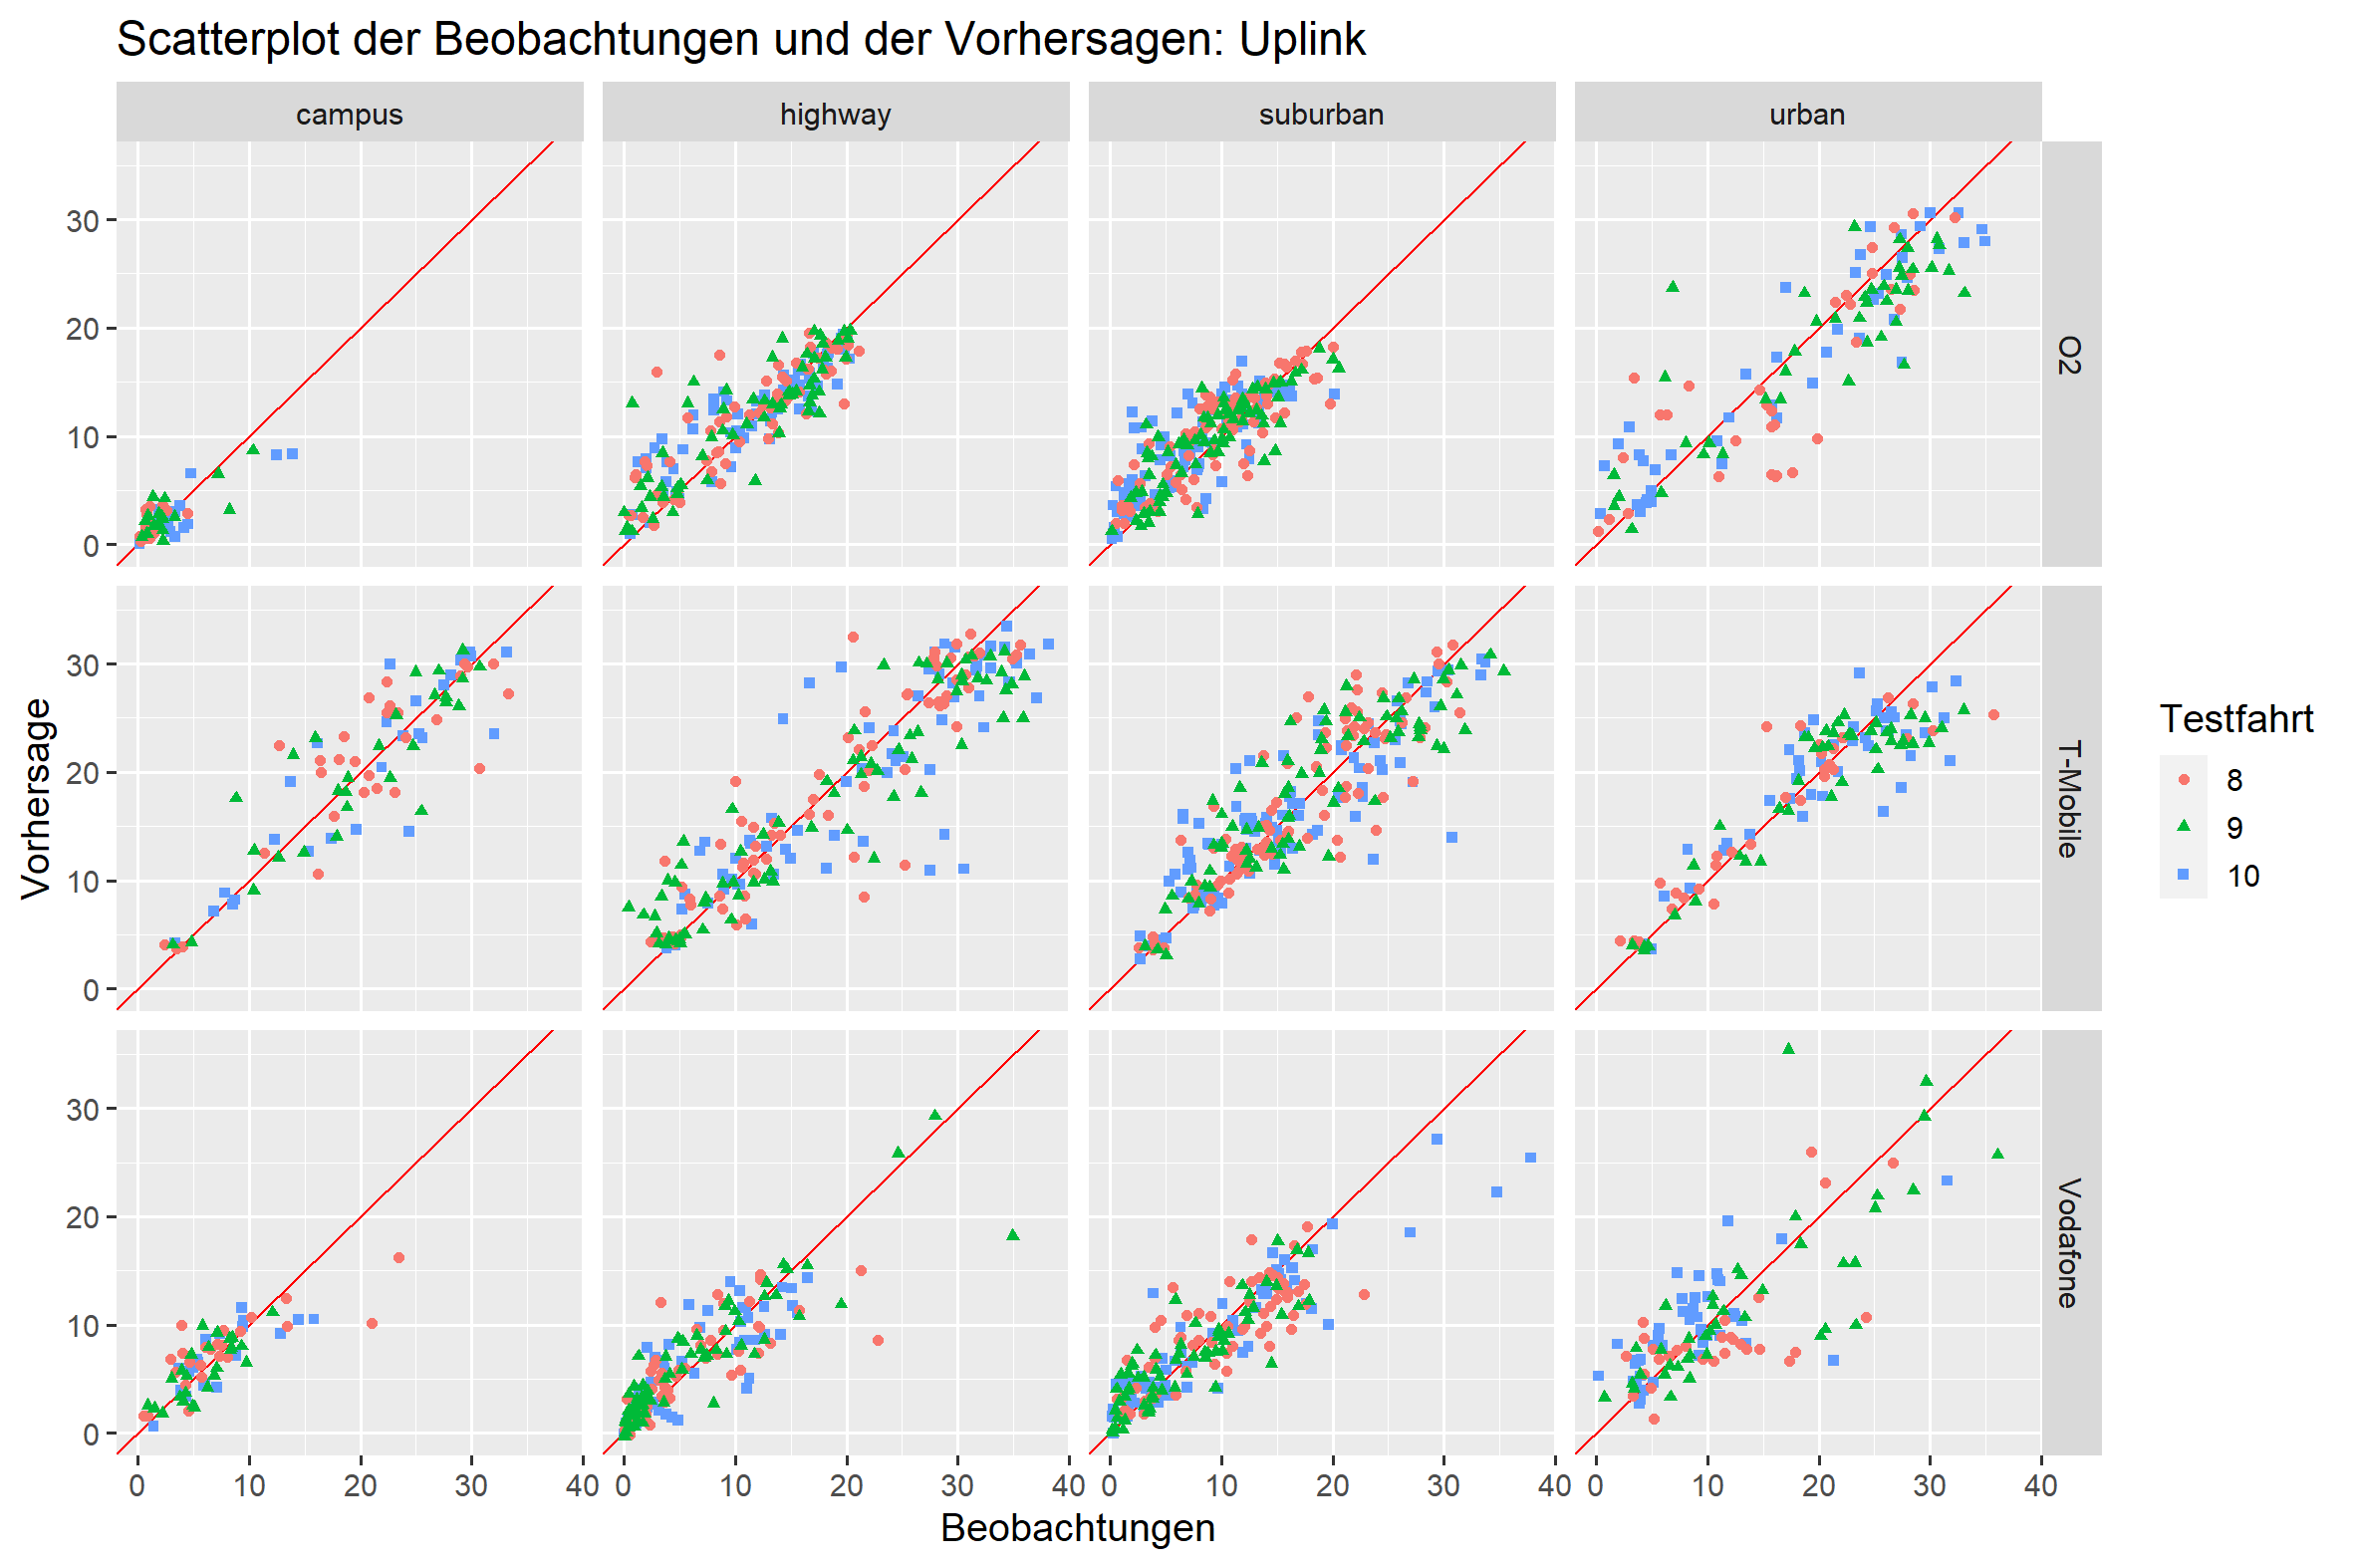
\includegraphics[scale=0.33]{plots/xgboost/uplink/scatter_colored_axes_fixed}
        \caption{XGBoost Out-of-Sample Vorhersagen der Upload-Rate}
        \label{xgboost_scatter_colored_uplink}
    \end{figure}
\end{frame}

\begin{frame}{Out-of-Sample Vorhersagen}
    \begin{figure}[h]
        \centering
        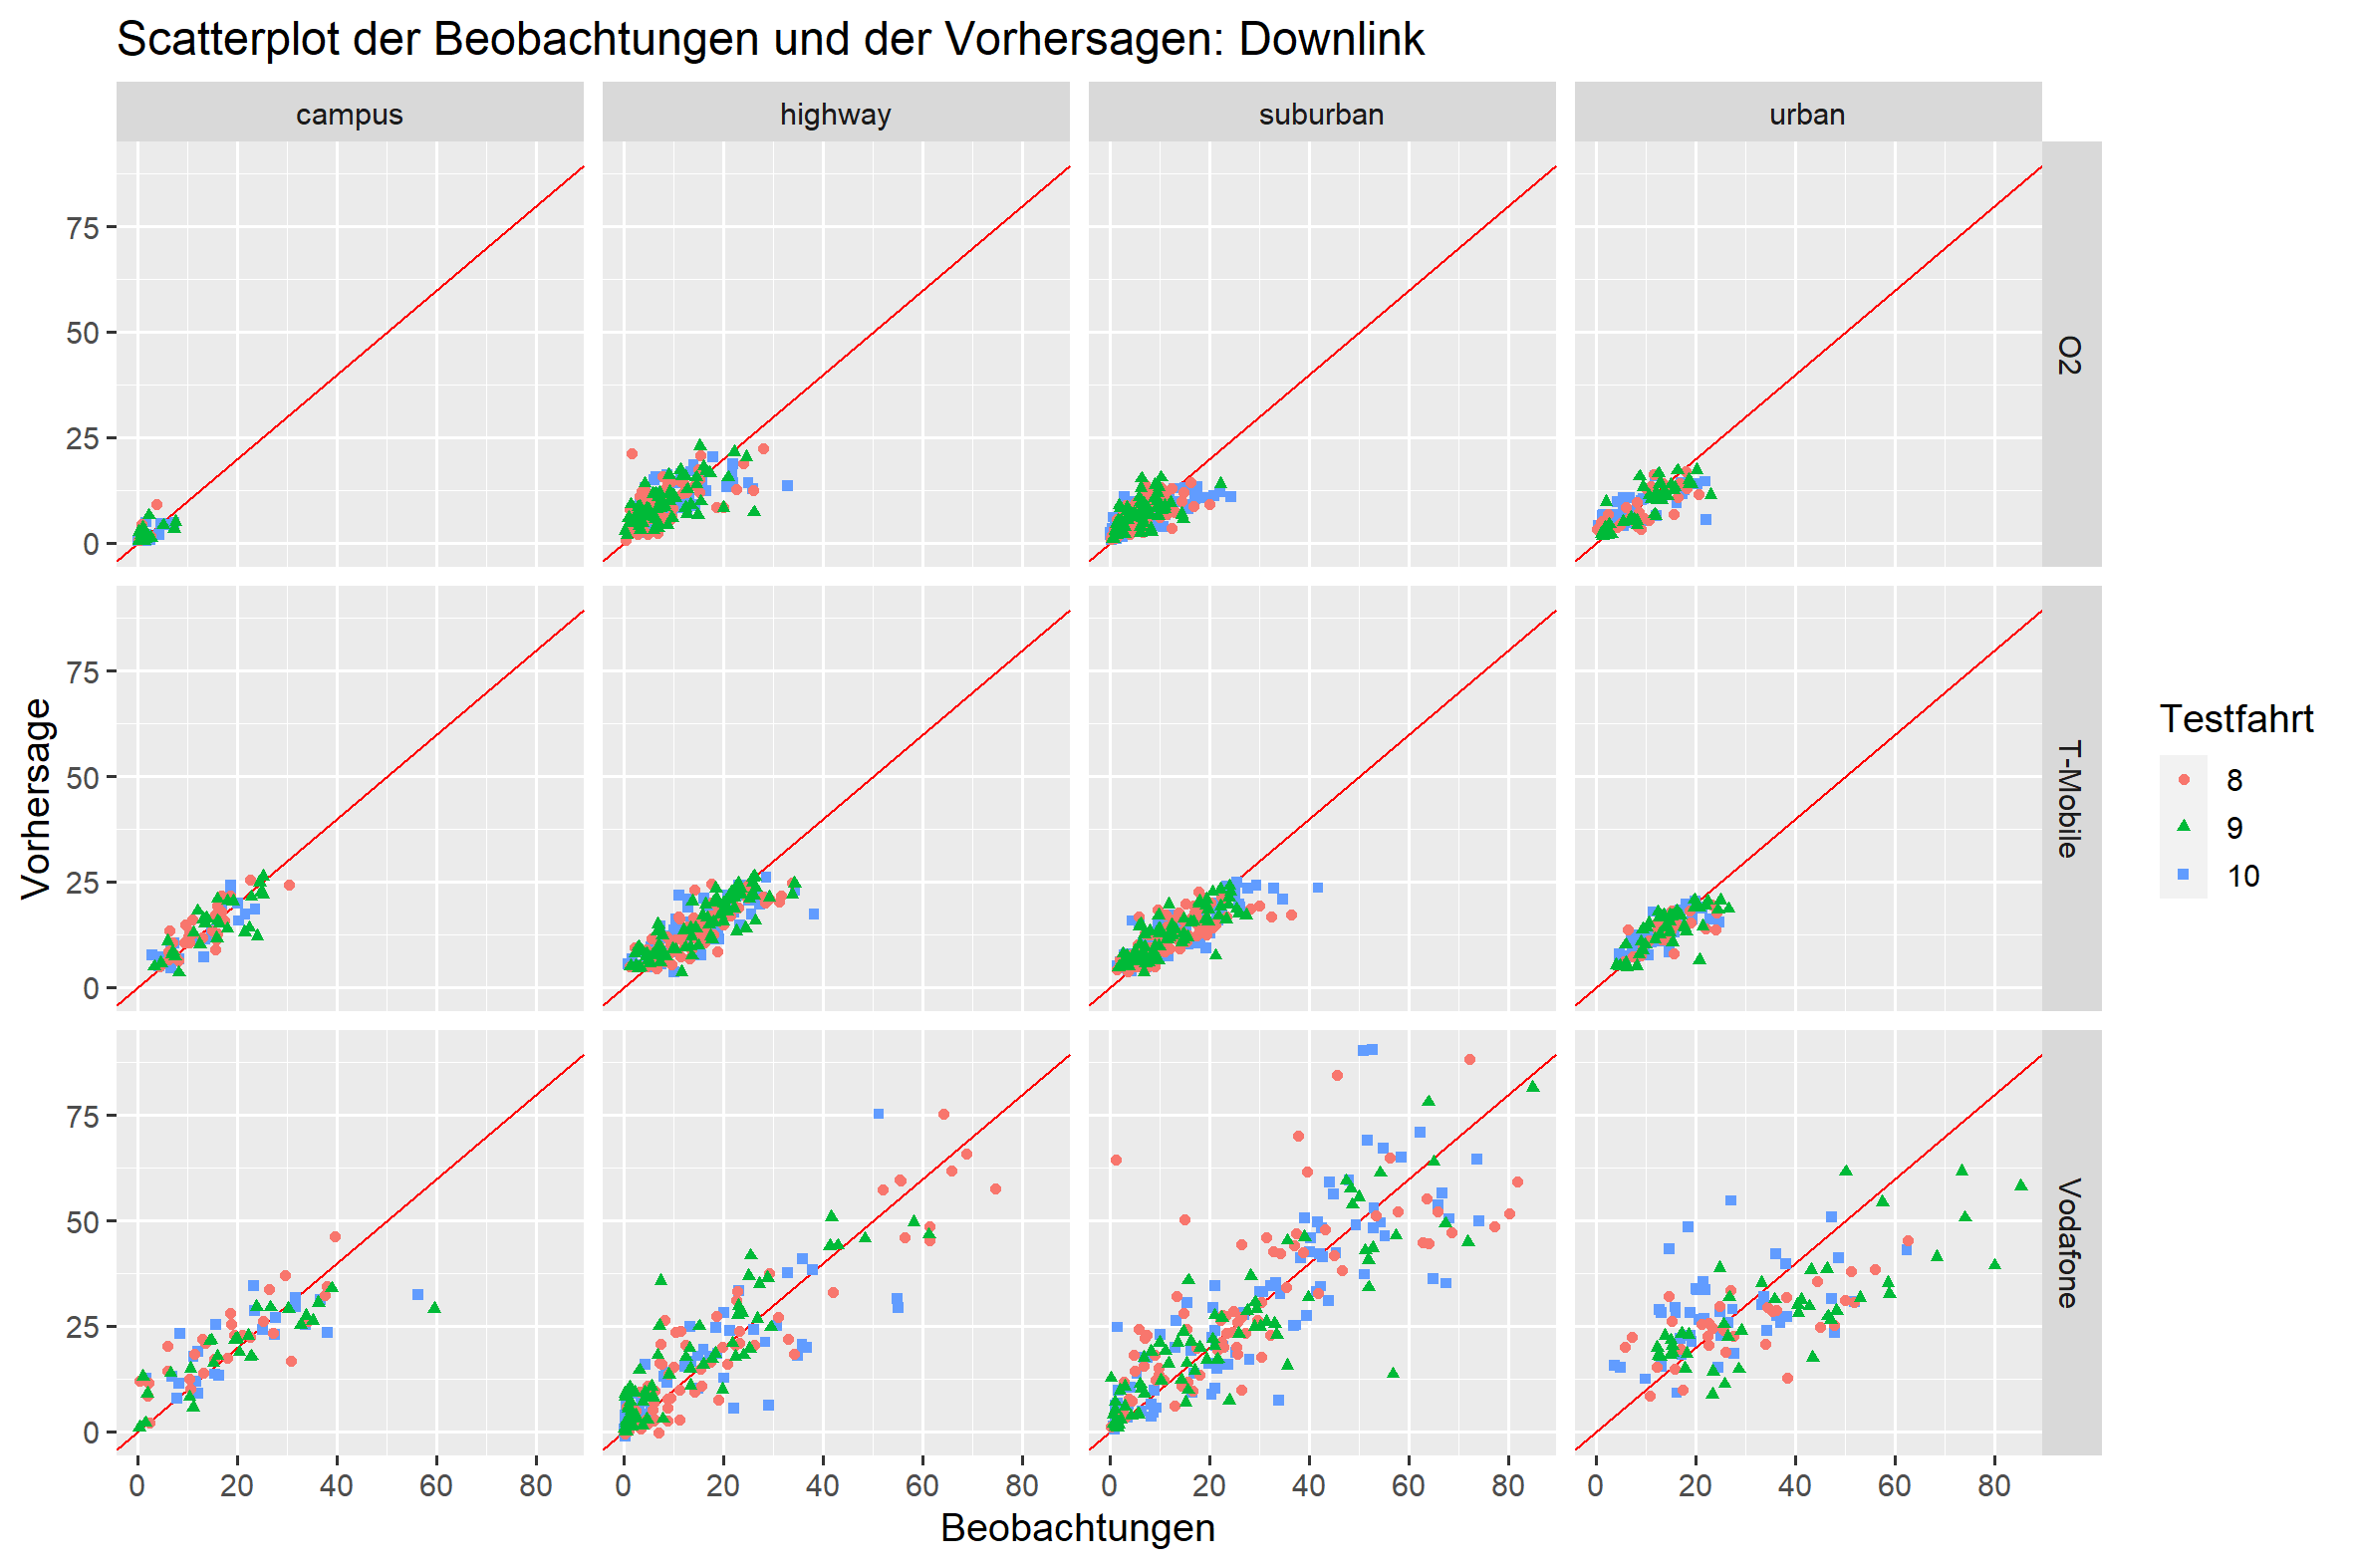
\includegraphics[scale=0.33]{plots/xgboost/downlink/scatter_colored_axes_fixed}
        \caption{XGBoost Out-of-Sample Vorhersagen der Download-Rate}
        \label{xgboost_scatter_colored_downlink}
    \end{figure}
\end{frame}